\documentclass[11pt,oneside]{article}    %use"amsart"insteadof"article"forAMSLaTeXformat
\usepackage{geometry}        %Seegeometry.pdftolearnthelayoutoptions.Therearelots.
\geometry{letterpaper}        %...ora4paperora5paperor...
%\geometry{landscape}        %Activateforforrotatedpagegeometry
%\usepackage[parfill]{parskip}        %Activatetobeginparagraphswithanemptylineratherthananindent
\usepackage{graphicx}                %Usepdf,png,jpg,orepsßwithpdflatex;useepsinDVImode
                                %TeXwillautomaticallyconverteps-->pdfinpdflatex        
\usepackage{amssymb}
\usepackage[colorlinks]{hyperref}

%----macros begin---------------------------------------------------------------
\usepackage{color}
\usepackage{amsthm}

\def\conv{\mbox{\textrm{conv}\,}}
\def\aff{\mbox{\textrm{aff}\,}}
\def\E{\mathbb{E}}
\def\R{\mathbb{R}}
\def\Z{\mathbb{Z}}
\def\tex{\TeX}
\def\latex{\LaTeX}
\def\v#1{{\bf #1}}
\def\p#1{{\bf #1}}
\def\T#1{{\bf #1}}

\def\vet#1{{\left(\begin{array}{cccccccccccccccccccc}#1\end{array}\right)}}
\def\mat#1{{\left(\begin{array}{cccccccccccccccccccc}#1\end{array}\right)}}

\def\lin{\mbox{\rm lin}\,}
\def\aff{\mbox{\rm aff}\,}
\def\pos{\mbox{\rm pos}\,}
\def\cone{\mbox{\rm cone}\,}
\def\conv{\mbox{\rm conv}\,}
\newcommand{\homog}[0]{\mbox{\rm homog}\,}
\newcommand{\relint}[0]{\mbox{\rm relint}\,}

%----macros end-----------------------------------------------------------------

\title{Accelerated intersection of geometric objects
\footnote{This document is part of the \emph{Linear Algebraic Representation with CoChains} (LAR-CC) framework~\cite{cclar-proj:2013:00}. \today}
}
\author{Alberto Paoluzzi}
%\date{}                            %Activatetodisplayagivendateornodate

\begin{document}
\maketitle
\nonstopmode

\begin{abstract}
This module contains the first experiments of a parallel implementation of the intersection of (multidimensional) geometric objects. The first installment is being oriented to the intersection of line segment in the 2D plane. A generalization of the algorithm, based on the classification of the containment boxes of the geometric values, will follow quickly.
\end{abstract}

\tableofcontents

%===============================================================================
\section{Introduction}
%===============================================================================

%===============================================================================
\section{Implementation}
%===============================================================================

\subsection{Basic operations}
%===============================================================================

\paragraph{Containment boxes}
%-------------------------------------------------------------------------------
@D Containment boxes
@{""" Containment boxes """
def containmentBoxes(randomLineArray):
    boxes = [eval(vcode([min(x1,x2),min(y1,y2),max(x1,x2),max(y1,y2)]))
            for ((x1,y1),(x2,y2)) in randomLineArray]
    return boxes
@}
%-------------------------------------------------------------------------------

\subsection{Construction of independent buckets}
%===============================================================================



\paragraph{Box metadata computation}
%-------------------------------------------------------------------------------
@D Box metadata computation
@{""" Box metadata computation """
def boxOrdering(boxes):
    boxes = [box+[k] for k,box in enumerate(boxes)]
    x1 = TRANS(sorted(boxes,key=S1))[4]
    y1 = TRANS(sorted(boxes,key=S2))[4]
    x2 = TRANS(sorted(boxes,key=S3,reverse=True))[4]
    y2 = TRANS(sorted(boxes,key=S4,reverse=True))[4]
    return x1,y1,x2,y2
@}
%-------------------------------------------------------------------------------


\paragraph{Splitting the input above and below a threshold}
%-------------------------------------------------------------------------------
@D Splitting the input above and below a threshold
@{""" Splitting the input above and below a threshold """
def splitOnThreshold(boxes,subset,x1,x2,xy='x'):
    theBoxes = [boxes[k] for k in subset]
    threshold = centroid(theBoxes,xy)
    if xy=='x': a=0;b=2;
    elif xy=='y': a=1;b=3;
    below,above = [],[]
    for k in subset:
        if boxes[k][a] <= threshold: below += [k]
    for k in subset:
        if boxes[k][b] >= threshold: above += [k]
    return below,above
@}
%-------------------------------------------------------------------------------


\paragraph{Iterative splitting of box buckets}
%-------------------------------------------------------------------------------
@D Iterative splitting of box buckets
@{""" Iterative splitting of box buckets """
def boxBuckets(boxes):
    x1,y1,x2,y2 = boxOrdering(boxes)
    bucket = range(len(boxes))
    splittingStack = [bucket]
    finalBuckets = []
    while splittingStack != []:
        bucket = splittingStack.pop()
        below,above = splitOnThreshold(boxes,bucket,x1,x2,'x')
        below1,above1 = splitOnThreshold(boxes,above,y1,y2,'y')
        below2,above2 = splitOnThreshold(boxes,below,y1,y2,'y')
        
        if (len(below1)<4 and len(above1)<4) or len(set(bucket).difference(below1))<7 \
            or len(set(bucket).difference(above1))<7: 
            finalBuckets.append(below1)
            finalBuckets.append(above1)
        else: 
            splittingStack.append(below1)
            splittingStack.append(above1)
            
        if (len(below2)<4 and len(above2)<4) or len(set(bucket).difference(below2))<7 \
            or len(set(bucket).difference(above2))<7:  
            finalBuckets.append(below2)
            finalBuckets.append(above2)
        else: 
            splittingStack.append(below2)
            splittingStack.append(above2)
    return list(set(AA(tuple)(finalBuckets)))
@}
%-------------------------------------------------------------------------------


\subsection{Brute force intersection within the buckets}
%===============================================================================




\paragraph{Intersection of two line segments}
%-------------------------------------------------------------------------------
@D Intersection of two line segments
@{""" Intersection of two line segments """
def segmentIntersect(pointStorage):
    def segmentIntersect0(segment1):
        p1,p2 = segment1
        line1 = '['+ vcode(p1) +','+ vcode(p2) +']'
        (x1,y1),(x2,y2) = p1,p2
        #B1,B2,B3,B4 = eval(vcode([min(x1,x2),min(y1,y2),max(x1,x2),max(y1,y2)]))
        def segmentIntersect1(segment2):
            p3,p4 = segment2
            line2 = '['+ vcode(p3) +','+ vcode(p4) +']'
            (x3,y3),(x4,y4) = p3,p4
            #b1,b2,b3,b4 = eval(vcode([min(x3,x4),min(y3,y4),max(x3,x4),max(y3,y4)]))
            #if ((B1<=b1<=B3) or (B1<=b3<=B3)) and ((B2<=b2<=B4) or (B2<=b4<=B4)):
            if True:
                m23 = mat([p2,p3])
                m14 = mat([p1,p4])
                m = m23 - m14
                v3 = mat([p3])
                v1 = mat([p1])
                v = v3-v1
                a=m[0,0]; b=m[0,1]; c=m[1,0]; d=m[1,1];
                det = a*d-b*c
                if det != 0:
                    m_inv = mat([[d,-b],[-c,a]])*(1./det)
                    alpha, beta = (v*m_inv).tolist()[0]
                    #alpha, beta = (v*m.I).tolist()[0]
                    if 0<=alpha<=1 and 0<=beta<=1:
                        pointStorage[line1] += [alpha]
                        pointStorage[line2] += [beta]
                        return list(array(p1)+alpha*(array(p2)-array(p1)))
            return None
        return segmentIntersect1
    return segmentIntersect0
@}
%-------------------------------------------------------------------------------


\paragraph{Brute force bucket intersection}
%-------------------------------------------------------------------------------
@D Brute force bucket intersection
@{""" Brute force bucket intersection """
def lineBucketIntersect(lines,pointStorage):
    intersect0 = segmentIntersect(pointStorage)
    intersectionPoints = []
    n = len(lines)
    for k,line in enumerate(lines):
        intersect1 = intersect0(line)
        for h in range(k+1,n):
            line1 = lines[h]
            point = intersect1(line1)
            if point != None: 
                intersectionPoints.append(eval(vcode(point)))
    return intersectionPoints
@}
%-------------------------------------------------------------------------------


\paragraph{Accelerate intersection of lines}
%-------------------------------------------------------------------------------
@D Accelerate intersection of lines
@{""" Accelerate intersection of lines """
def lineIntersection(lineArray):

    from collections import defaultdict
    pointStorage = defaultdict(list)
    for line in lineArray:
    	p1,p2 = line
    	key = '['+ vcode(p1) +','+ vcode(p2) +']'
    	pointStorage[key] = []

    boxes = containmentBoxes(lineArray)
    buckets = boxBuckets(boxes)
    intersectionPoints = set()
    for bucket in buckets:
        lines = [lineArray[k] for k in bucket]
        pointBucket = lineBucketIntersect(lines,pointStorage)
        intersectionPoints = intersectionPoints.union(AA(tuple)(pointBucket))

    frags = AA(eval)(pointStorage.keys())
    params = AA(COMP([sorted,list,set,tuple,eval,vcode]))(pointStorage.values())
        
    return intersectionPoints,params,frags  ### GOOD: 1, WRONG: 2 !!!
@}
%-------------------------------------------------------------------------------



\paragraph{Create the LAR of fragmented lines}
%-------------------------------------------------------------------------------
@D Create the LAR of fragmented lines
@{""" Create the LAR of fragmented lines """
def lines2lar(lineArray):
    intersectionPoints,params,frags = lineIntersection(lineArray)
    vertDict = dict()
    index,defaultValue,V,EV = -1,-1,[],[]
    
    for k,(p1,p2) in enumerate(frags):
        outline = [vcode(p1)]
        if params[k] != []:
            for alpha in params[k]:
                if alpha != 0.0 and alpha != 1.0:
                    p = list(array(p1)+alpha*(array(p2)-array(p1)))
                    outline += [vcode(p)]
        outline += [vcode(p2)]
    
        edge = []
        for key in outline:
            if vertDict.get(key,defaultValue) == defaultValue:
                index += 1
                vertDict[key] = index
                edge += [index]
                V += [eval(key)]
            else:
                edge += [vertDict[key]]
        EV.extend([[edge[k],edge[k+1]] for k,v in enumerate(edge[:-1])])
    return V,EV
@}
%-------------------------------------------------------------------------------

%===============================================================================
\section{Exporting the module}
%===============================================================================

%-------------------------------------------------------------------------------
@O lib/py/inters.py
@{""" Module for pipelined intersection of geometric objects """
from pyplasm import *
""" import modules from larcc/lib """
import sys
sys.path.insert(0, 'lib/py/')
from larcc import *
DEBUG = True

@< Coding utilities @>
@< Generation of random lines @>
@< Containment boxes @>
@< Splitting the input above and below a threshold @>
@< Box metadata computation @>
@< Iterative splitting of box buckets @>
@< Intersection of two line segments @>
@< Brute force bucket intersection @>
@< Accelerate intersection of lines @>
@< Create the LAR of fragmented lines @>
@}
%-------------------------------------------------------------------------------


%===============================================================================
\section{Examples}
%===============================================================================




\paragraph{Generation of random line segments and their boxes}
%-------------------------------------------------------------------------------
@O test/py/inters/test01.py
@{""" Generation of random line segments and their boxes """
import sys
sys.path.insert(0, 'lib/py/')
from inters import *

randomLineArray = randomLines(200,0.3)
VIEW(STRUCT(AA(POLYLINE)(randomLineArray)))

boxes = containmentBoxes(randomLineArray)
rects= AA(box2rect)(boxes)
cyan = COLOR(CYAN)(STRUCT(AA(POLYLINE)(randomLineArray)))
yellow = COLOR(YELLOW)(STRUCT(AA(POLYLINE)(rects)))
VIEW(STRUCT([cyan,yellow]))
@}
%-------------------------------------------------------------------------------


\paragraph{Split segment array in four independent buckets}
%-------------------------------------------------------------------------------
@O test/py/inters/test02.py
@{""" Split segment array in four independent buckets """
import sys
sys.path.insert(0, 'lib/py/')
from inters import *

randomLineArray = randomLines(200,0.3)
VIEW(STRUCT(AA(POLYLINE)(randomLineArray)))
boxes = containmentBoxes(randomLineArray)
x1,y1,x2,y2 = boxOrdering(boxes)
bucket = range(len(boxes))
below,above = splitOnThreshold(boxes,bucket,x1,x2,'x')
below1,above1 = splitOnThreshold(boxes,above,y1,y2,'y')
below2,above2 = splitOnThreshold(boxes,below,y1,y2,'y')

cyan = COLOR(CYAN)(STRUCT(AA(POLYLINE)(randomLineArray[k] for k in below1)))
yellow = COLOR(YELLOW)(STRUCT(AA(POLYLINE)(randomLineArray[k] for k in above1)))
red = COLOR(RED)(STRUCT(AA(POLYLINE)(randomLineArray[k] for k in below2)))
green = COLOR(GREEN)(STRUCT(AA(POLYLINE)(randomLineArray[k] for k in above2)))

VIEW(STRUCT([cyan,yellow,red,green]))
@}
%-------------------------------------------------------------------------------



\paragraph{Generation of independent line buckets}
%-------------------------------------------------------------------------------
@O test/py/inters/test03.py
@{""" Generation of independent line buckets """
import sys
sys.path.insert(0, 'lib/py/')
from inters import *

lines = randomLines(200,0.3)
VIEW(STRUCT(AA(POLYLINE)(lines)))

boxes = containmentBoxes(lines)
buckets = boxBuckets(boxes)

colors = [CYAN, MAGENTA, WHITE, RED, YELLOW, GRAY, GREEN, ORANGE, BLACK, BLUE, PURPLE, BROWN]
sets = [COLOR(colors[k%12])(STRUCT(AA(POLYLINE)([lines[h] 
            for h in bucket]))) for k,bucket in enumerate(buckets)]

VIEW(STRUCT(sets))
@}
%-------------------------------------------------------------------------------


\paragraph{Generation of independent line buckets}
%-------------------------------------------------------------------------------
@O test/py/inters/test04.py
@{""" Generation of independent line buckets """
import sys
sys.path.insert(0, 'lib/py/')
from inters import *

lines = randomLines(400,0.2)
VIEW(STRUCT(AA(POLYLINE)(lines)))

intersectionPoints,params,frags = lineIntersection(lines)

marker = CIRCLE(.005)([4,1])
markers = STRUCT(CONS(AA(T([1,2]))(intersectionPoints))(marker))
VIEW(STRUCT(AA(POLYLINE)(lines)+[COLOR(RED)(markers)]))

V,EV = lines2lar(lines)
#markers = STRUCT(CONS(AA(T([1,2]))(V))(marker))
markers = STRUCT(CONS(AA(T([1,2]))(intersectionPoints))(marker))
polylines = STRUCT(MKPOLS((V,EV)))
VIEW(STRUCT([polylines]+[COLOR(MAGENTA)(markers)]))
@}
%-------------------------------------------------------------------------------


\paragraph{Splitting of othogonal lines}
%-------------------------------------------------------------------------------
@O test/py/inters/test05.py
@{""" Splitting of othogonal lines """
import sys
sys.path.insert(0, 'lib/py/')
from inters import *

lines = [
[[0,0],[6,0]],
[[0,4],[6,4]],
[[0,0],[0,4]],
[[3,0],[3,4]],
[[6,0],[6,4]],
[[3,2],[6,2]]
]
VIEW(EXPLODE(1.2,1.2,1)(AA(POLYLINE)(lines)))

V,EV = lines2lar(lines)
VIEW(EXPLODE(1.2,1.2,1)(MKPOLS((V,EV))))
@}
%-------------------------------------------------------------------------------

\begin{figure}[htbp] %  figure placement: here, top, bottom, or page
   \centering
   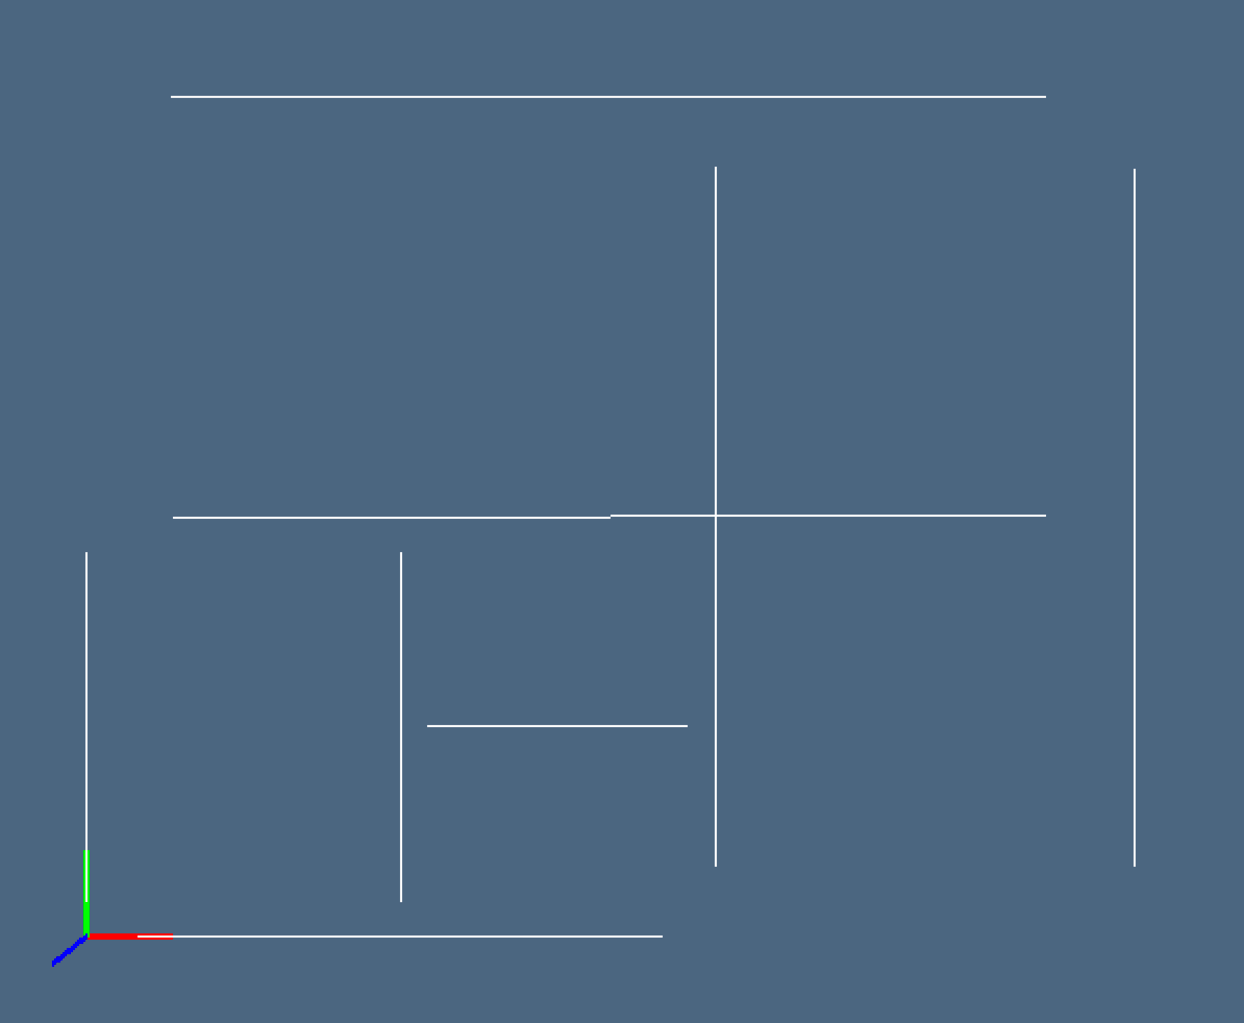
\includegraphics[width=0.49\linewidth]{images/ortho1} 
   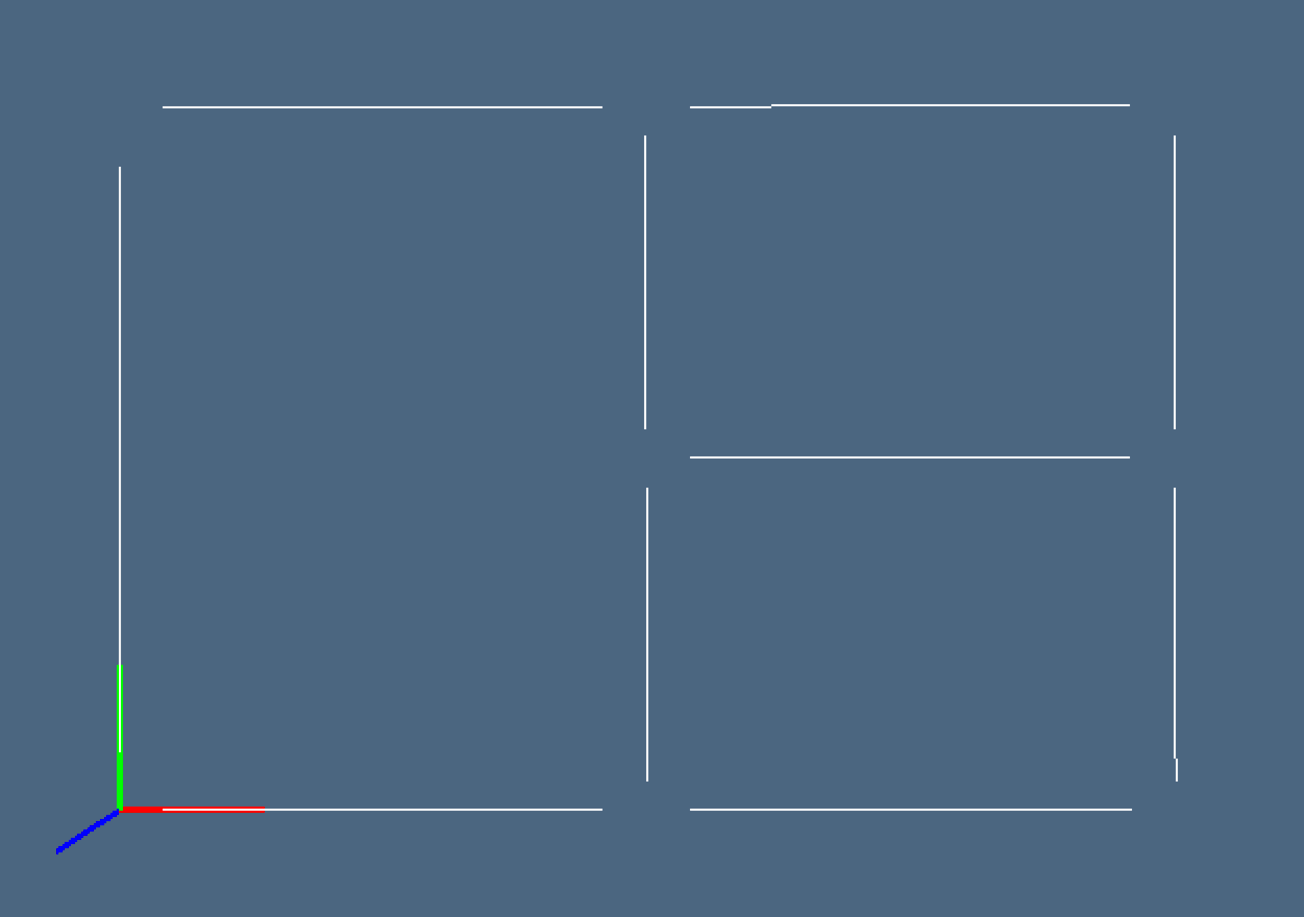
\includegraphics[width=0.49\linewidth]{images/ortho2} 
   \caption{Splitting of othogonal lines: (a) exploded input; (a) exploded output.}
   \label{fig:ortho}
\end{figure}



\paragraph{Random coloring of the generated 1-complex}
%-------------------------------------------------------------------------------
@O test/py/inters/test06.py
@{""" Random coloring of the generated 1-complex """
import sys
sys.path.insert(0, 'lib/py/')
from inters import *

lines = randomLines(400,0.2)
VIEW(STRUCT(AA(POLYLINE)(lines)))

V,EV = lines2lar(lines)
colors = [CYAN, MAGENTA, WHITE, RED, YELLOW, GRAY, GREEN, ORANGE, BLACK, BLUE, PURPLE, BROWN]
sets = [COLOR(colors[k%12])(POLYLINE([V[e[0]],V[e[1]]])) for k,e in enumerate(EV)]

VIEW(STRUCT(sets))
@}
%-------------------------------------------------------------------------------

\begin{figure}[htbp] %  figure placement: here, top, bottom, or page
   \centering
   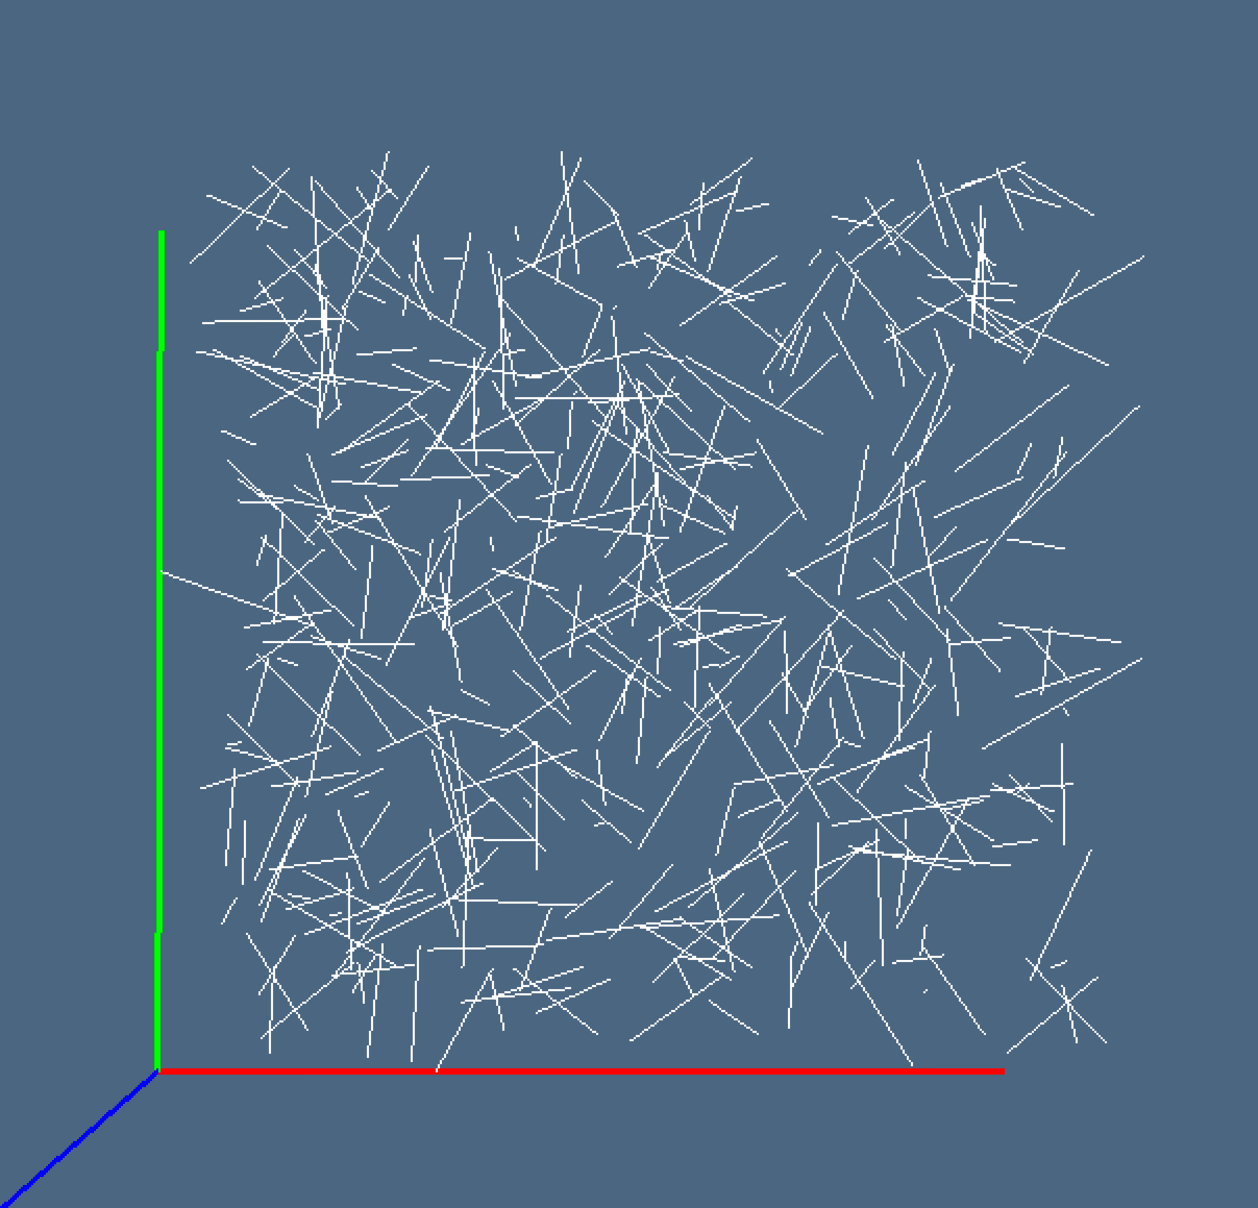
\includegraphics[width=0.49\linewidth]{images/colored1} 
   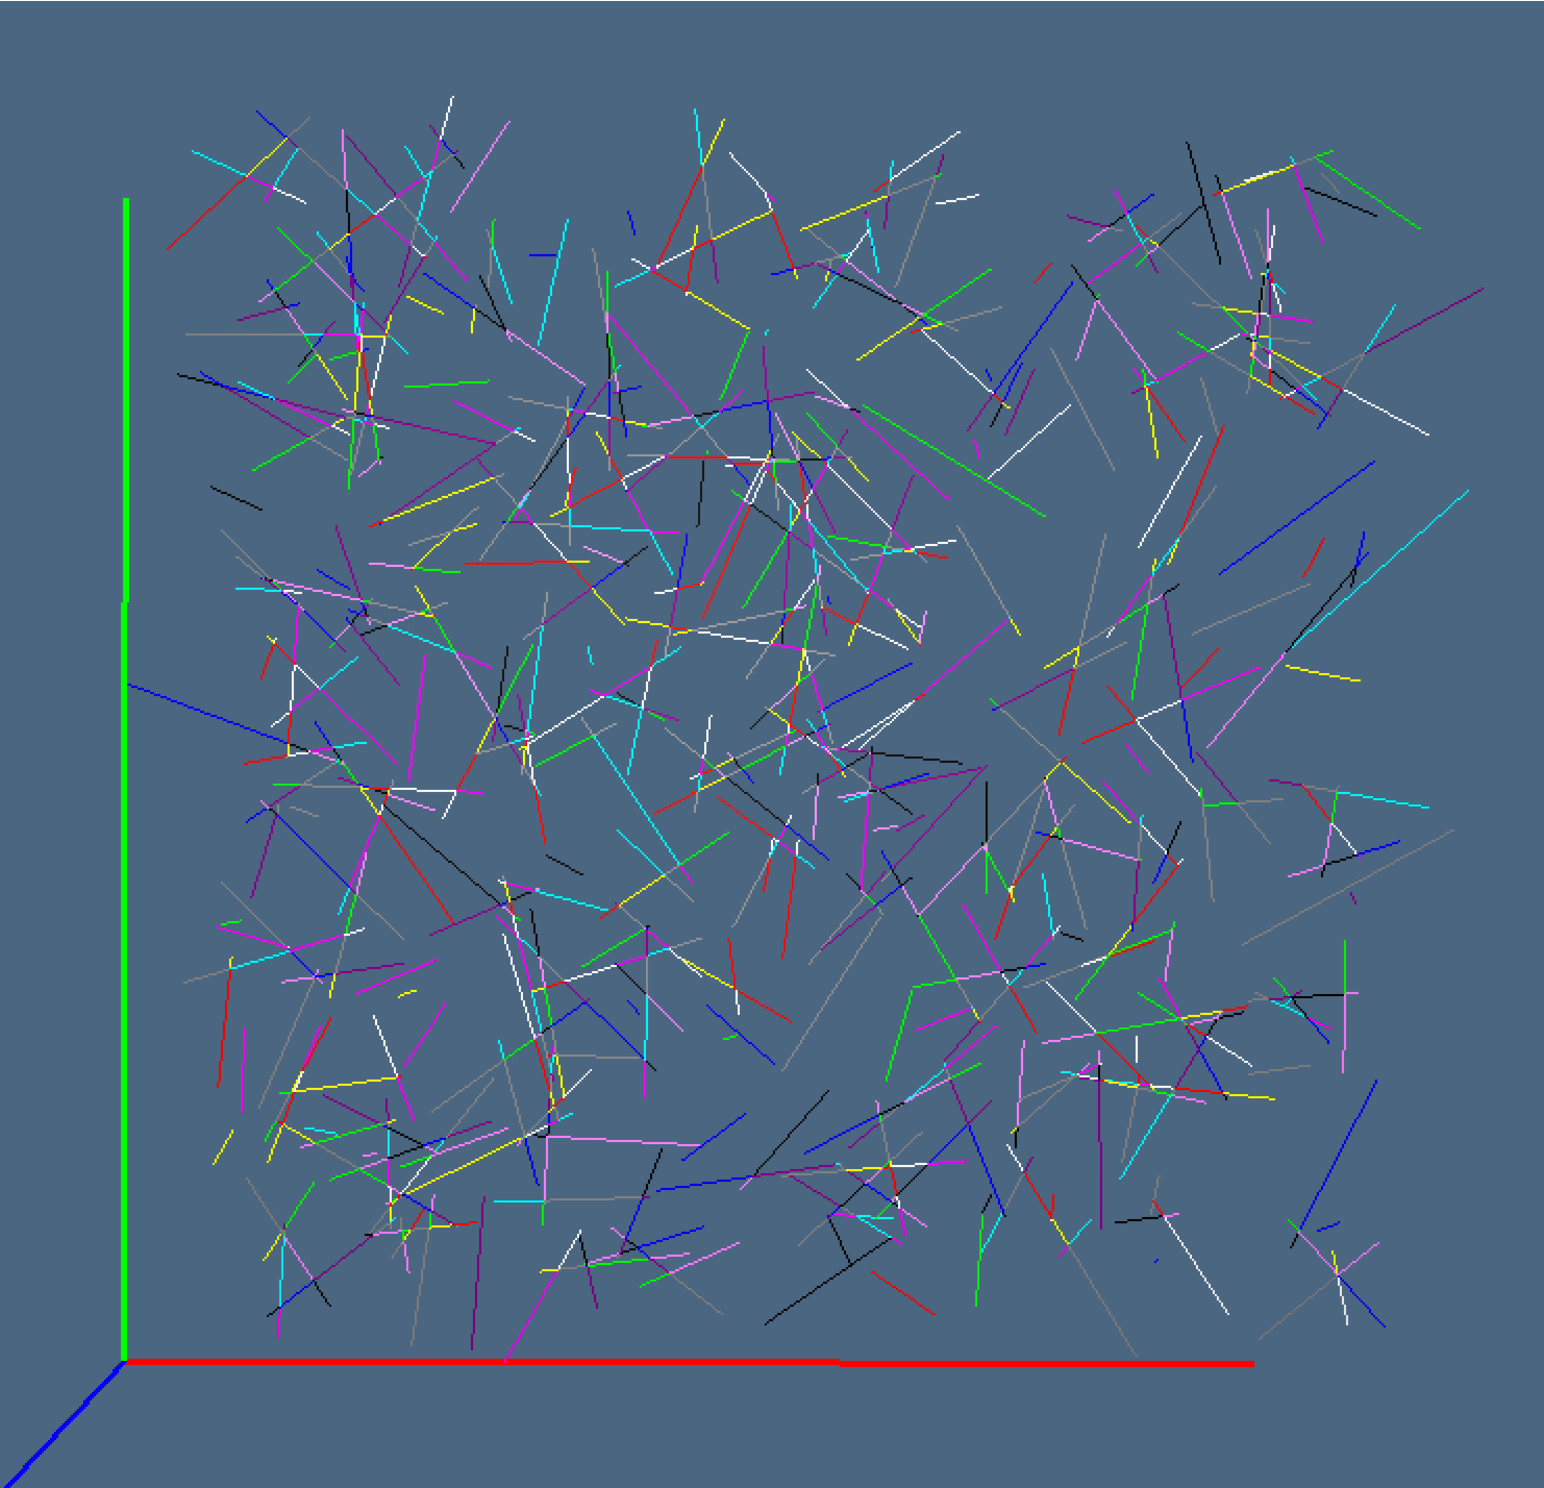
\includegraphics[width=0.49\linewidth]{images/colored2} 
   \caption{Splitting of intersecting lines: (a) random input; (a) splitted and colored LAR output.}
   \label{fig:ortho}
\end{figure}



\begin{figure}[htbp] %  figure placement: here, top, bottom, or page
   \centering
   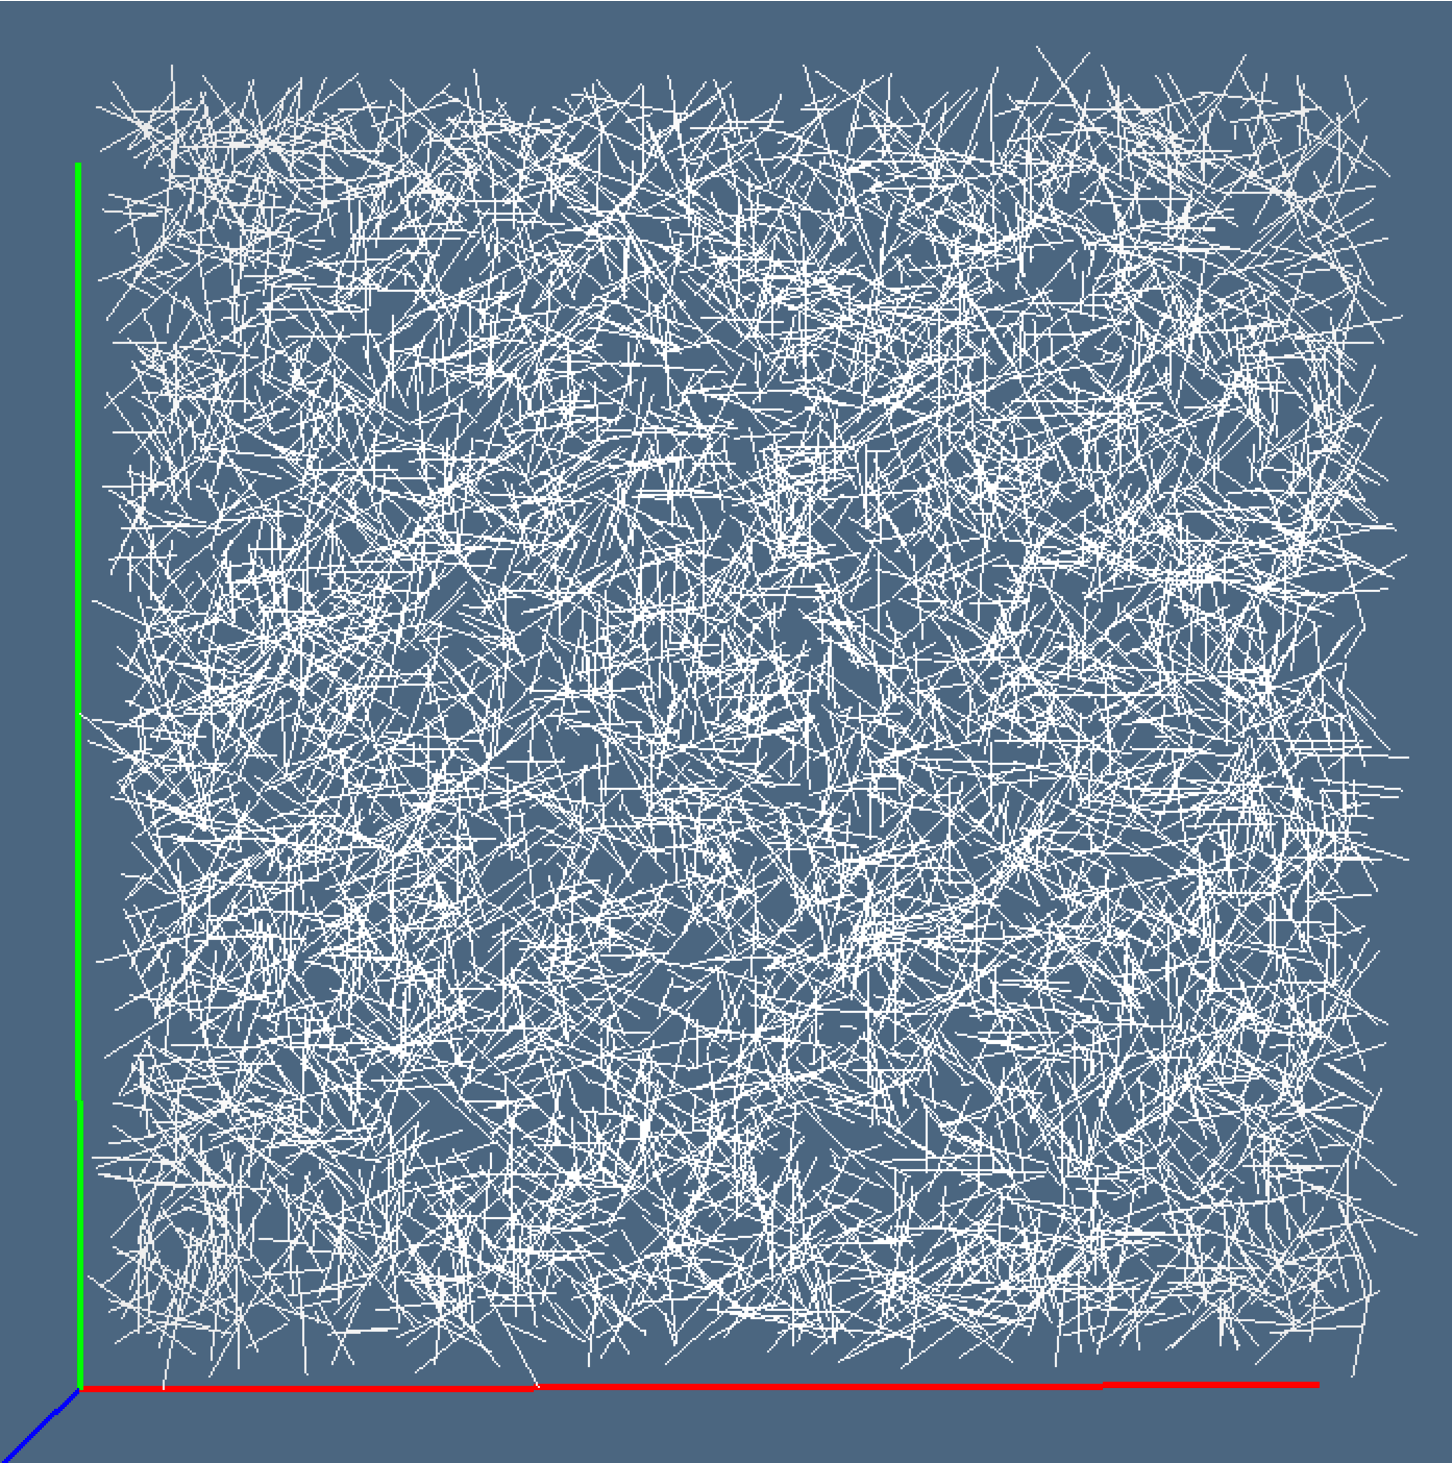
\includegraphics[height=0.49\linewidth,width=0.49\linewidth]{images/lineintersect1} 
   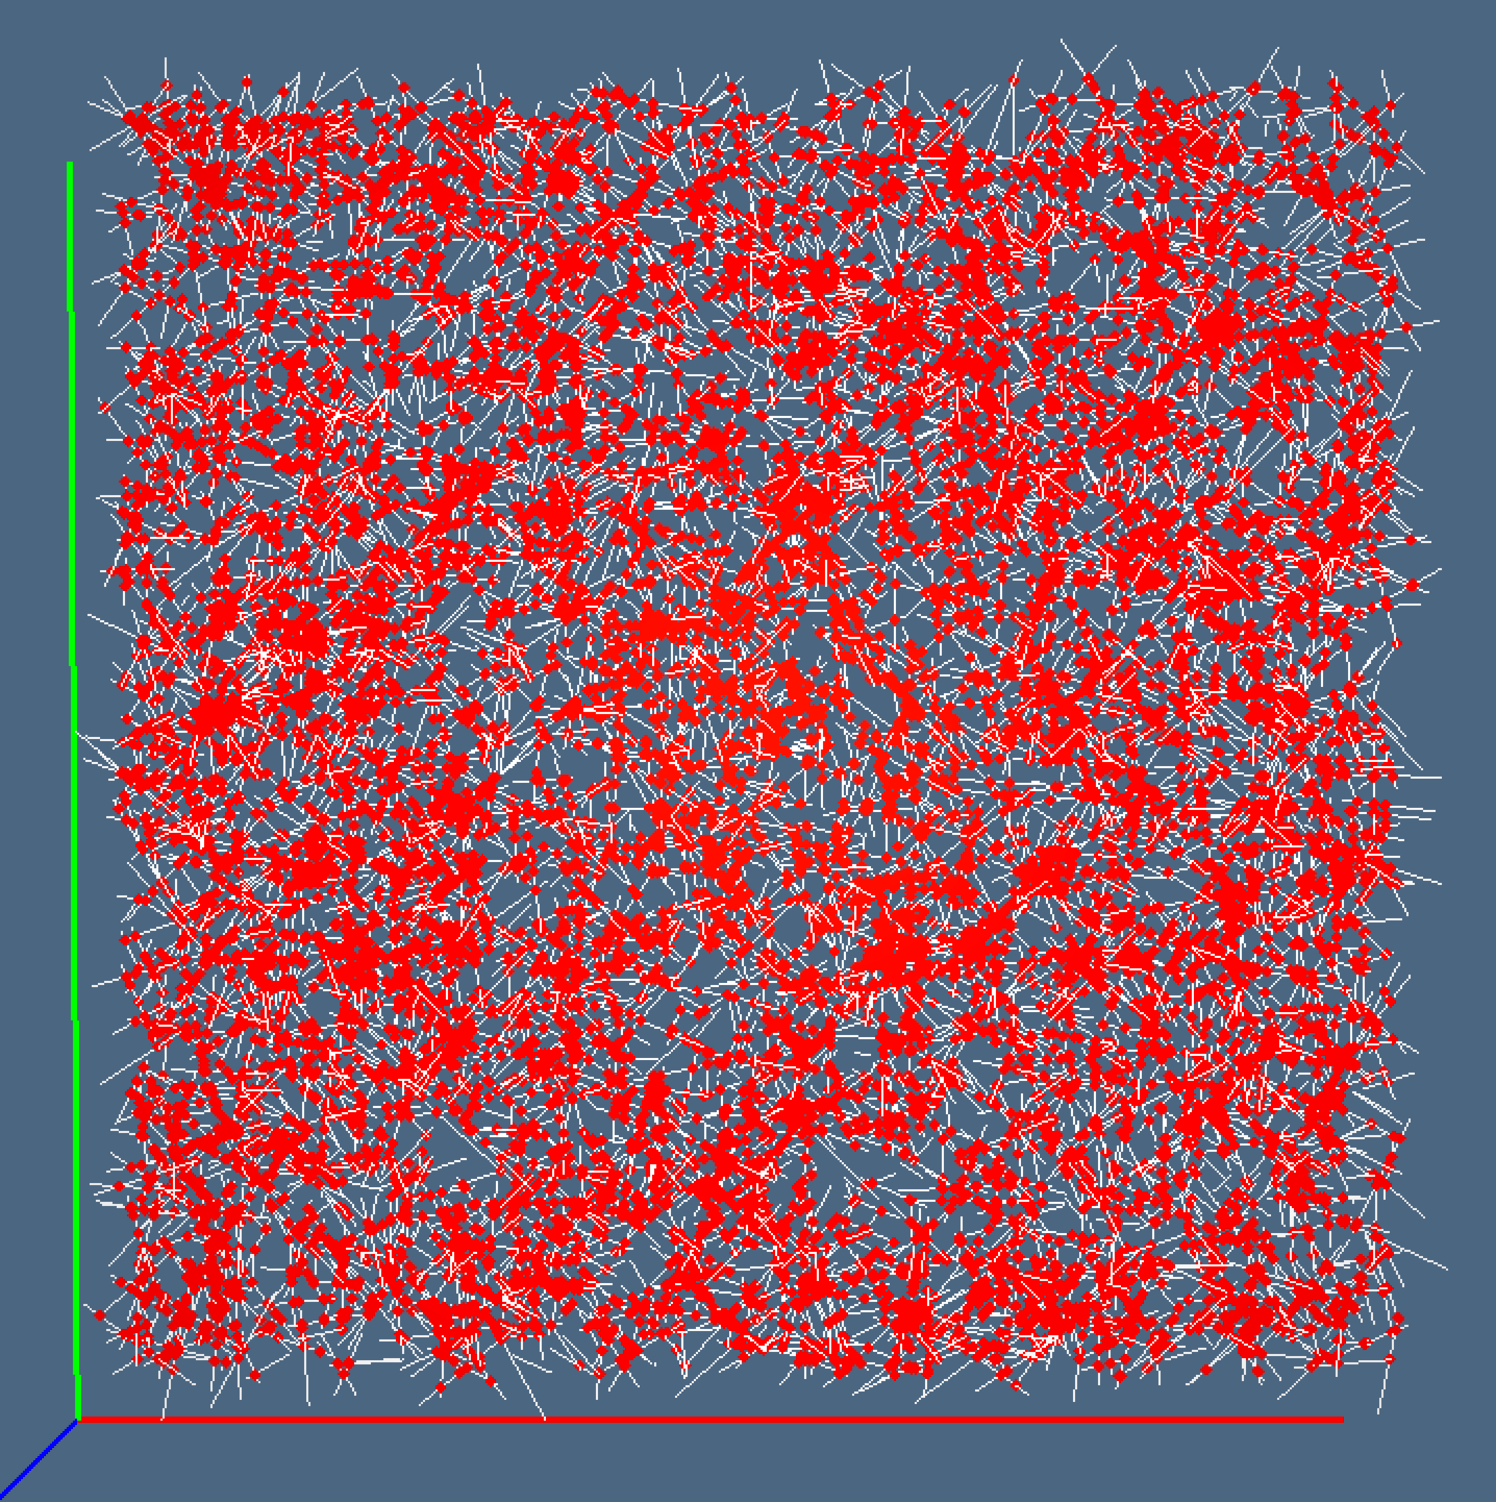
\includegraphics[height=0.49\linewidth,width=0.49\linewidth]{images/lineintersect2} 
   \caption{The intersection of 5000 random lines in the unit interval, with \texttt{scaling} parameter equal to \texttt{0.1}}
   \label{fig:example}
\end{figure}


\appendix
%===============================================================================
\section{Code utilities}
%===============================================================================

\paragraph{Coding utilities}
%-------------------------------------------------------------------------------
@D Coding utilities
@{""" Coding utilities """
@< Generation of a random point @>
@< Generation of a random line segment @>
@< Transformation of a 2D box into a closed polyline @>
@< Computation of the 1D centroid of a list of 2D boxes @>
@}
%-------------------------------------------------------------------------------


\paragraph{Generation of random lines}
%-------------------------------------------------------------------------------
@D Generation of random lines
@{""" Generation of random lines """
def randomLines(numberOfLines=200,scaling=0.3):
    randomLineArray = [redge(scaling) for k in range(numberOfLines)]
    [xs,ys] = TRANS(CAT(randomLineArray))
    xmin, ymin = min(xs), min(ys)
    v = array([-xmin,-ymin])
    randomLineArray = [[list(v1+v), list(v2+v)] for v1,v2 in randomLineArray]
    return randomLineArray
@}
%-------------------------------------------------------------------------------


\paragraph{Generation of a random point}
%-------------------------------------------------------------------------------
@D Generation of a random point
@{""" Generation of a random point """
def rpoint():
    return eval( vcode([ random.random(), random.random() ]) )
@}
%-------------------------------------------------------------------------------
    
\paragraph{Generation of a random line segment}
%-------------------------------------------------------------------------------
@D Generation of a random line segment
@{""" Generation of a random line segment """
def redge(scaling):
    v1,v2 = array(rpoint()), array(rpoint())
    c = (v1+v2)/2
    pos = rpoint()
    v1 = (v1-c)*scaling + pos
    v2 = (v2-c)*scaling + pos
    return tuple(eval(vcode(v1))), tuple(eval(vcode(v2)))
@}
%-------------------------------------------------------------------------------
    
\paragraph{Transformation of a 2D box into a closed polyline}
%-------------------------------------------------------------------------------
@D Transformation of a 2D box into a closed polyline
@{""" Transformation of a 2D box into a closed polyline """    
def box2rect(box):
    x1,y1,x2,y2 = box
    verts = [[x1,y1],[x2,y1],[x2,y2],[x1,y2],[x1,y1]]
    return verts
@}
%-------------------------------------------------------------------------------
    
\paragraph{Computation of the 1D centroid of a list of 2D boxes}
%-------------------------------------------------------------------------------
@D Computation of the 1D centroid of a list of 2D boxes
@{""" Computation of the 1D centroid of a list of 2D boxes """    
def centroid(boxes,xy='x'):
    delta,n = 0,len(boxes)
    if xy=='x': a=0; b=2
    elif xy=='y': a=1; b=3
    for box in boxes:
        delta += (box[a] + box[b])/2
    return delta/n
@}
%-------------------------------------------------------------------------------


\bibliographystyle{amsalpha}
\bibliography{inters}

\end{document}
